\chapter{Technology Review} \label{techreview}
This chapter will cover the technical side of our project, by looking back on the technologies that made up the final revision of the project. We will explain the different technologies we added and how they were implemented through the project. We will look over the web stack we used and the technologies we added in order to create a more robust and useful social media site. We will go over why we used the given technologies and the benefits we saw in them over others.

% ========================== Framework  ========================== 
\section{MEAN STACK/Framework} \label{meanstack}
The mean stack is intended to provide a simple and fun starting point for cloud native full-stack JavaScript applications. MEAN is a set of Open Source components that together, provide an end-to-end framework for building dynamic web applications; starting from the top (code running in the browser) to the bottom (database). 

The stack is made up of:

\begin{itemize}
\item MongoDB
\item ExpressJS
\item Angular
\item Node.js
\end{itemize}

Early in development when we were brainstorming, we decided to do a full stack development. The next step after this decision was to figure out how to carry out this task. We looked into full development stacks such as the MERN stack (MongoDB, ExpressJS, React, Node.js), MEAN stack (MongoDB, ExpressJS, Angular, Node.js) or doing a Java-based development stack (Spring boot, Angular, MongoDB). After lots of discussion and input from supervisors, we decided to not go with the Java-based development stack. We then took a deep dive into the difference between the MEAN/MERN stack to decide what route we wanted to take and start development as soon as possible. After looking into React JSX vs Angular HTML templating and experimenting with the two stacks we finally decided that the MEAN stack was more inline in what we wanted to learn.

Once we knew what stack we were using and how to use it in a basic form from our prototyping stage, we moved onto breaking the stack down to each component and getting to know each component better, so when full development starts we would have a better understand how the entire stack operates and interacts with each component. This gave us a greater understanding of how each component operated and allowed us to plan out how each component would operate from top to bottom. 

\subsection{MongoDB}
You may know what MySQL and other relational databases are. MySQL is analogous to a spreadsheet, it has name columns and rows of rows of data. Every database "tool" shows the data as a spreadsheet (Microsoft Access). Data can be linked through special functions such as a "JOIN" mechanism to allow the user to built meta spreadsheets. 

MongoDB is a database and not a database tool (Mongo Compass), instead of a spreadsheet like MySQL it is more like a folder of documents. The contents of the "folders" are not checked to see if the new file differs from the current file format. This sounds like an inefficient system but all these folders are called collections in MongoDB. The collections are usually grouped by how the user would group MySQL tables. While MongoDB can contain keys like MySQL there is no built-in functionality in order to join documents together in order to retrieve related data in another collection.

Databases are classified into two categories of SQL and NoSQL. MySQL is an example of an SQL database, and MongoDB is an example of a NoSQL database. MongoDB is very reliable as its very hands off and gives the user the responsibility for how data is saved and read. If a user adds another entry into the collection that doesn't match the other entries MongoDB doesn't inform the user that the data is not in the correct format as collections do not have definitions and leave that responsibility to the user. The same goes for joining two collections together. The joining is left up to the user on how they carry that out, usually, the user would create an ID which is present in both collections in order to 'join' them together.

MongoDB is so hands off about how users read and write to the database it stops the frequently used attack on SQL databases called SQL injection. SQL injection occurs when the user directly interacts with the database which allows them to manipulate their input to test the database. MongoDB doesn't have this problem as its hands off the reading data to the user to the point where a search for that data will include the statement but nor process the statement as such.

MongoDB uses the JSON standard to store data. The JSON data is then classified into a collection as we discussed above. 

Example of how a JSON entry in a collection could look like:

\begin{minted}{js}
{
    "username": "Smithy",
    "password": "smith123",
    "name": {
        "first_name" : "John",
        "second_name" : "Smith",
    }
}
\end{minted}

\subsection{ExpressJS}
ExpressJS is a minimalistic web framework built for Node.js that waits for the browser to connect so the server can send process the request and send back the relevant form (JSON, HTML, Raw Text, ETC...). Without ExpressJS the user must handle creating a server, handling routing all manually.

ExpressJS relies on APIs made available by Node.js. ExpressJS cannot exist without Node.js. ExpressJS is a thin layer over Node.js which makes developing servers and routes much easier. ExpressJS's main feature that makes it enticing to developers is how it serves dynamic content (Content that changes based on user requests). 

ExpressJS also has the capability to server components from frameworks such as Angular, Ember and React and process requests made by those components to update their content. ExpressJS makes Node.js development easier, especially when creating APIs that front-end apps use. Express makes it easier to unify the front-end apps and the API.

ExpressJS was an easy pick for the project as it easily integrates Node.js and rapidly decreased the time it would take to get the server side API up and running.

\subsection{Angular}
Angular is a front-end web framework built on top of JavaScript, it is used to develop single-page web applications. Single-page web frameworks (Angular, React, Ember) are websites which have all the functionality of a multiple page website without having the need to refresh the browser when moving from page to page. Single-page web development frameworks have become increasingly popular in the last few years due to how reactive they are. Pages react very fast and fluidly making user interaction with the website more positive than refreshing when moving to another page on the same website. 

Angular has been around since 2010 with the release of AngularJS. Later version came out and greatly improved upon the idea with Angular 2+ or Angular v2. This version would be improved upon and maintained by Google with the latest release being Angular 7 in late 2018. Despite angular being around for nearly 10 years, it has only been in the last few years where it has come into its own and seen real competition from other single-page frameworks such as React and Ember.

We chose Angular because of its integration with Node.js/ExpressJS which allowed us to get prototypes for testing the MEAN stack up and running very quickly and let us play around with the different functions it offered as part of its component-based setup. Within a week we had the entire MEAN stack in a functional state where Angular was served with Node.js/ExpressJS and then send and received data from the API served by the Node.js/ExpressJS server.

\subsection{Node.js}
Node.js is a cross-platform JavaScript run-time environment that allows developers to run JavaScript outside the browser. This framework is a huge deal for JavaScript. Node.js allows developers to perform actions with JavaScript on the developer's local machine like they would with other programming languages. What makes Node.js so beloved by developers is the built-in functionality of Node.js. Node.js has built-in HTTP function to allow Node.js to run HTTP actions all within the environment. This built-in HTTP functionality has made Node.js extremely popular and given the rise to isomorphic web applications and due to the fact that Node.js can run as a server back-end using JavaScript and have JavaScript on the front-end meaning there is the opportunity for the two to share code between them reducing testing and maintenance.

Node.js is a great framework due when paired with a front-end framework such as Angular, and a database such as MongoDB. When using a setup like this the entire web stack is a JavaScript based and allows the user to easily manipulate data from top to bottom.

The reason we picked Node.js is because of its ease of use and how rapidly we could get a working HTTP server up and running. Node.js also made a lot of sense when paired with Angular which was the front-end framework we picked. Node.js makes developing HTTP servers easy, which allowed us to spend more time on setting up other features such as user authentication and the Reddit API. 

Here is an example of all the code needed to create a simple Node.js server. This code will display "Hello World!" to the user in the browser on port "8080".
\begin{minted}{js}
var http = require('http');

//create a server object:
http.createServer(function (req, res) {
  res.write('Hello World!');
  res.end();
}).listen(8080);
\end{minted}

\subsubsection{Node Modules}
Node.js allows developers to develop and use packages which provide the developer with more functionality.

\begin{figure}[H]
  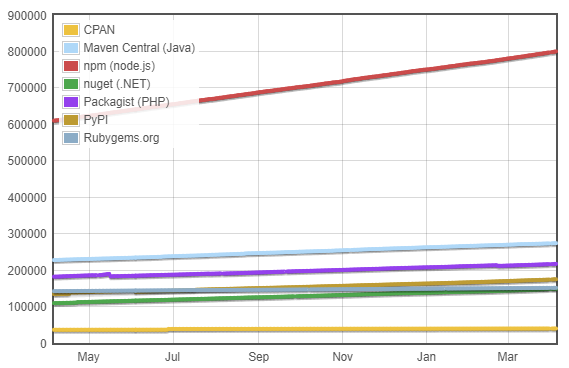
\includegraphics[width=\linewidth]{img/moduleCount.PNG}
  \caption{NPM Package Count}
  \label{fig:NPM}
\end{figure}

NPM is the world’s largest software registry. NPM allows developers access to lots of packages for all sorts of development such as packages for Node.js, Angular, MongoDB and even developing Alexa skills. NPM allows developers to upload custom packages that they have developed and give access to other developers to use it in their system.

Node modules is a powerful resource with lots of packages that adds great functionality to the developer's project such as user authentication with Passport.js.

% ========================== DEPLOYMENT  ========================== 
\section{Deployment}
For code deployments we looked at numerous cloud service provides to figure out what would be the best service to take use of for our project. We looked at Google Cloud, Heroku and AWS as the cloud service providers. Although these are only a fraction of the cloud service providers online, we found they were received very well by our supervisors as a way of deployment. 

We ruled out Google cloud after lots of debate on how to move forward with deployment. The reason to remove Google Cloud first was we felt that we wanted to get a greater understanding of a different cloud service provider as we already had experience with Google Cloud. After ruling our Google Cloud we were left with Heroku and AWS. After researching more into both options and figuring out what would better with our project we decided to go with AWS because of AWS's Elastic Beanstalk. AWS Elastic Beanstalk is a system provided by AWS for deploying and scaling web applications and services developed with Java, .NET, PHP, Node.js, Python, Ruby, Go, and Docker on familiar servers.  Because of AWS's Elastic Beanstalk and us using the MEAN stack, it was an easy way to deploy our project, and an easier way to expand the project if we wanted to go commercial with the website.

% ========================== STANDARDS  ========================== 
\section{Standards}
\subsection{JSON}
JavaScript Object-Notation is a specification for Serialization a data object. Serialization is a is the process that turns a price of code into a string of characters in order to transmit it. 

The basic idea is that if you want to transmit a piece of data that has attributes such as name, address, age, etc and turning it into a string.

An example of converting an object to JSON specification would be for example this object of the user.

\begin{minted}{java}
class user{
    string username;
    string password;
    int age;
}
\end{minted}

Let's say the user created an instance of this object and set the values to "Smithy", "smith123" and "25". To send this instance over to another machine in a standard the other machine we can't just send it in raw text using HTTP so we need to serialize the data before transfer using the JSON specification. 

The JSON string would look like this when the class is serialized:
\begin{minted}{js}
{
    "username": "Smithy",
    "password": "smith123",
    "age": 25
}
\end{minted}

Once the class is correctly serialized, the object can be added to the HTTP request to be sent over to the other machine. The JSON object would be added to the body of the HTTP request for the machine on the other end to retrieve and do with as it needs.

An example of it in the body would be:
\begin{minted}{js}
{ "user": {"username": "Smithy","password": "smith123","age": 25} }
\end{minted}

With this machine-readable string, I can now retrieve the data by deserializing the string back into an object. This all works because of the JSON specification which creates a standard for how to serialize and deserialize the JSON object.

\subsection{REST}
Representational State Transfer or REST is a guideline for sending information on the Internet. It is an architectural system that has gained in popularity over the years. RESTful web services are a common way of accessing an online API. Users can make multiple different requests through one URL with certain parameters. The REST architecture design has an emphasis on nouns to tell what the resource the user is trying to access is and how the resource is going to be affected by HTTP modules. 

Let's say a developer is making a system that accesses a database that requires read, write, update and delete functions. A REST URL could be for example "/api/account". Using this URL we can create a RESTful resource that the developer has access to with all these functions.

Using the REST specification we can create these four functions in the one URL route or resource by using the different HTTP methods (GET, POST, PUT, DELETE) for each function. All four HTTP requests to do with a user account would use the "/api/account" route to read, write, update and delete the user's data.

The REST specification streamlines the development of a server API and makes managing the API on the server as well as the application using the API much easier.

% ========================== REST API  ========================== 
\section{REST API}
The REST API we setup is intended to give access to all aspects of the project in a public format. The REST API is used by Angular which gives the user a visual representation of the data being sent and received by the REST API. Some routes are protected by Passport.js which encodes user data used to access certain routes such as update profile picture or password.

A big benefit of the API is all functionality of the application is available from the REST API. This allows for us to if we decided to, add a mobile application or create a monitoring tool to see the data and analyze it.

\subsection{Security}
Routes altering data (POST, PUT, DELETE) requires the user to be authenticated to prevent data being altered by another user. We authenticated certain routes such as create a post to check who is creating this post, and to link to their profile but also so only they can post in their name. Authenticating routes such as comment, post, settings and following was a big part of the planning stage as we needed to figure out a way to stop intrusive behaviour from outside sources abusing the API.

To add a layer of security to user requests and ensure no malicious requests are made by other user trying to impersonate another user we added a Node.js import called PassportJS. PassportJS is authentication middle-ware for Node.js. PassportJS allows

\subsection{Swagger}
Swagger is an open source software framework sponsored by SmartBear. Swagger is used to create, document and consume  RESTful Web services. Swagger offers an easy way to document RESTful Web services by using Swagger documentation definitions and Swagger UI to document an API and give example on how the API works. Swagger works by having the developer add comments similar to java-docs in order to document a route telling swagger the components of the route and the model it uses. Giving swagger this information swagger will use the data to create a JSON object with all the data about the API in a format that can be used by the developer for other means or to be used in conjunction with swagger UI, which we will discuss later.

\subsubsection{Swagger.json}
As we discussed above Swagger is used to document a route. But how does it do that? Swagger creates a JSON object which it hosts at a given route in order to be accessible by developers for their own purposes, or by using Swagger UI.

The JSON part of Swagger is where the swagger documentation is rendered into a machine readable format.

\begin{minted}{js}
{
    info: { 
        title: "Node Swagger API",
        version: "1.0.0",
        description: "Api file for swagger"
    },
    host: "34.243.30.50:3000",
    basePath: "/",
    swagger: "2.0",
    paths: {},
    definitions: {},
    responses: { },
    parameters: { },
    securityDefinitions: { }
}
\end{minted}

Above is an example from the hosted project on AWS. As we can see this is a very basic model for without any route or definitions. Swagger includes basic information about the API such as the host and general Swagger information such as version and title. Swagger includes the host and base-path used by the API, with a list of definitions and paths about each API route.

\begin{minted}{js}
paths: {
    /api: {
        get: {
        tags: [
            "books"
            ],
            description: "Returns all books",
            produces: [
            "application/json"
            ],
            responses: {
                200: {
                    description: "An array of books",
                    schema: {
                        \$ref: "#/definitions/book"
                    }
                }
            }
        },
    },
},
\end{minted}

An example of one of the paths contained in the paths object array. In paths we have a list of paths documented using Swagger, these paths contain information about the path such as the title in which the path could be classified under, example above is 'Books'. With the title we can classify different paths that may handle something to do with 'books' and thus we may want to organizes the paths under 'books'. The path also contains the schema used which is very important in order to understand how the API route operates. Does the path return JSON?, XML?, raw text?

\begin{minted}{js}
definitions: {
    book: {
        properties: {
            isbn: {
                type: "string"
            },
            title: {
                type: "string"
            },
            author: {
                type: "string"
            },
            description: {
                type: "string"
            },
            published_year: {
                type: "string"
            },
            publisher: {
                type: "string"
            }
        }
    }
},
\end{minted}

Using the definition in conjunction with the path we can get a better picture of how to API route works and what data is needed for it to operate correctly. The definitions contains definitions for each route and each definition inside definitions contains properties which describe the routes data and what type of data each property is.

\subsubsection{Swagger UI}
Swagger UI is a visual representation of the API documented using Swagger. Swagger UI is a great as it enables developers to save a lot of time in documenting an API, as it uses the Swagger JSON to visualize the API. 

\begin{figure}[H]
  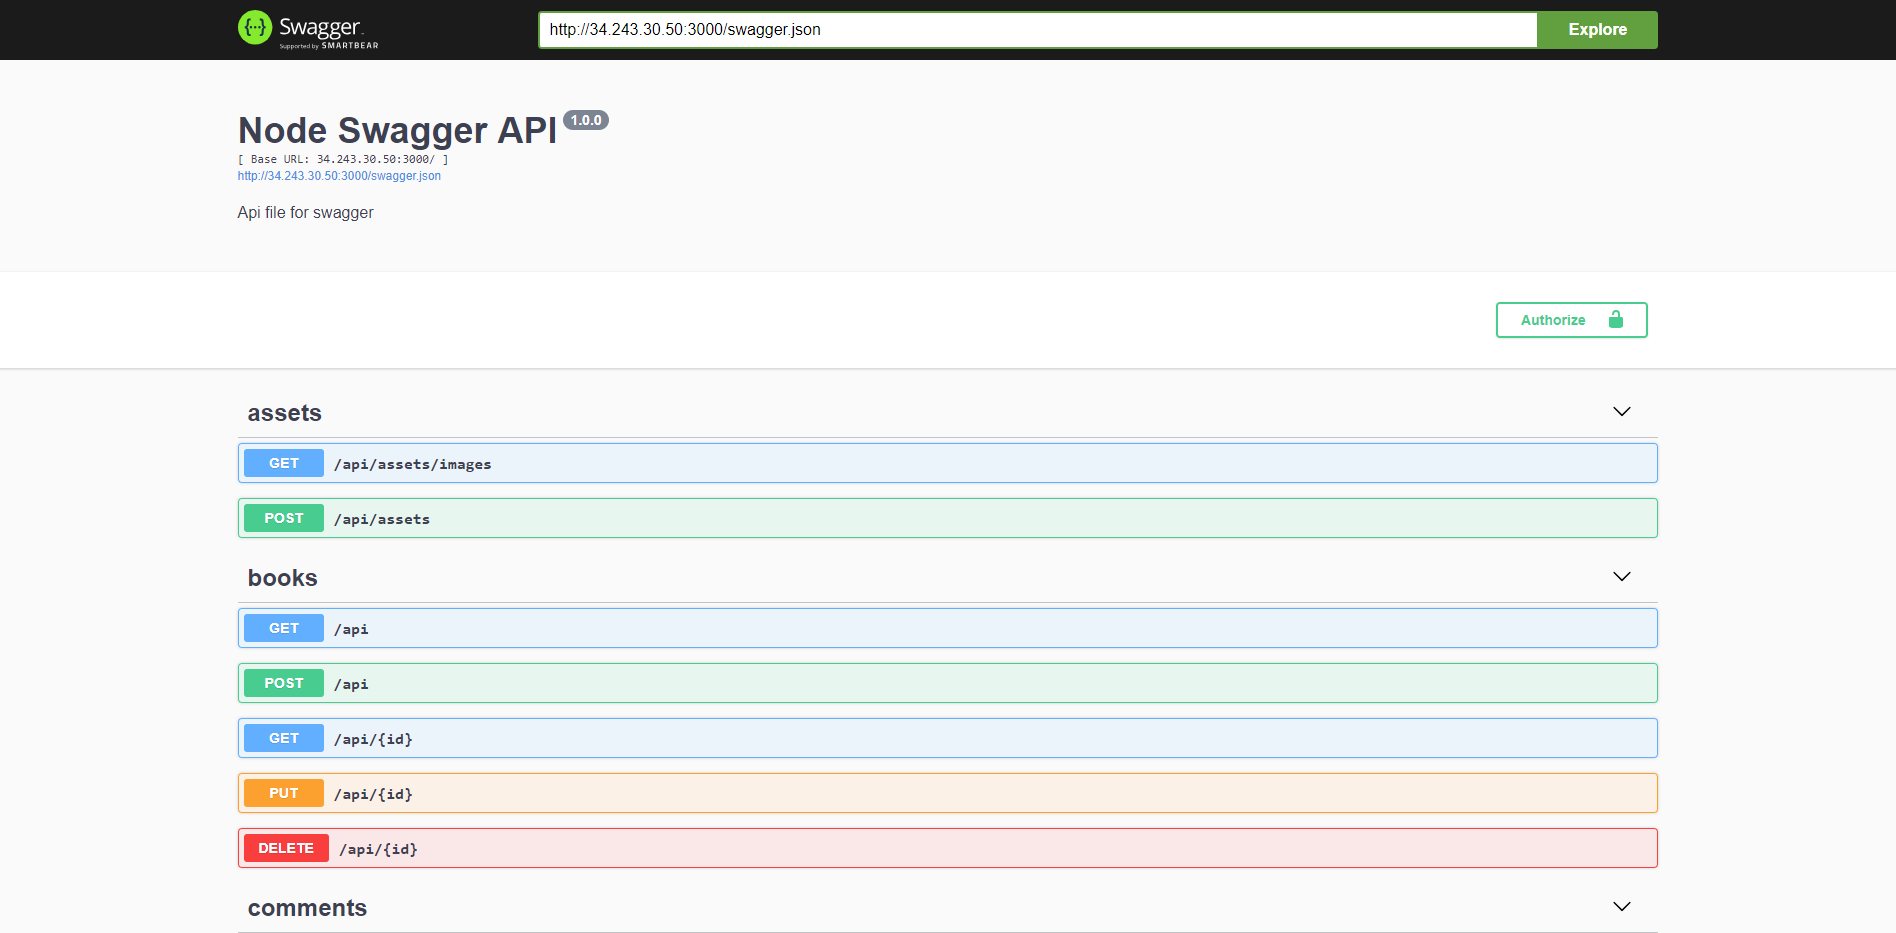
\includegraphics[width=\linewidth]{img/swaggerUI.PNG}
  \caption{Swagger UI}
  \label{fig:NPM}
\end{figure}

Using Swagger UI we can use the hosted JSON from the Swagger Documentation to display the available routes in the API. Each route is categorized and sorted using the Swagger JSON. Each option under the category will use the path and definition of the Swagger JSON to create a visualized representation of the API and allow testing of the API.

% ========================== Languages ========================== 
\section{Languages}
\subsection{JavaScript}
JavaScript is the backbone of the web. JavaScript is responsible for front-end web development processes. Without JavaScript a web page would have no functionality to communicate with the server-side functions in order to save or read dynamic data. JavaScript runs the web, both front-end with JavaScript or TypeScript. 

A very basic way to think of JavaScript is that HTML is your bone structure. It holds everything together with a solid foundation. CSS is your skin, it's what everyone sees and interacts with. So JavaScript is your brain, heart and other organs that make you, you. JavaScript is what makes everything function in an effective way.

\subsubsection{Database}
JavaScript is found in the database with MongoDB, which stores data using JSON (JavaScript Object Notation). MongoDB saves database entries using JSON to store elements of that collection. As we explained earlier what JSON is and how it stores classes into objects.

\subsubsection{Server-Side}
On the server-side we used Node.js. Node.js as we discussed above is what allows JavaScript to run outside the browser. JavaScript was used as the serer-side processing which handled routing for the API and for the Angular front-end.

\subsubsection{Front-End}
The front end section of the web application uses TypeScript which is a super-set of JavaScript which we will talk about in greater detail below.

in the server-side API handling routing for the web application. 

\subsection{TypeScript}
TypeScript which is a super-set of JavaScript. JavaScript code is valid in a TypeScript environment, with some exceptions. A huge benefit over JavaScript is that TypeScript made it harder to create bugs and made JavaScript more manageable in larger systems.

\vspace{5mm}

JavaScript:
\begin{minted}{js}
let name = 'TechBook',
users = 500,
isThreeTier = true;
\end{minted}

TypeScript:
\begin{minted}{js}
let name: string = 'TechBook',
users: number = 500,
isThreeTier: boolean = true;
\end{minted}

The biggest change and most liked feature of TypeScript is variables are declared by using a variable type such as 'string', 'number' and 'boolean'. This is a big change over JavaScript where the variable type is interpreted as to how the developer manages the variable.

\subsection{HTML}
HTML (Hypertext Markup Language) is a markup language for creating web pages. HTML uses tags to define what sections of the web page do what. 

HTML Example:
\begin{minted}{html}
<h1> Title </h1>
<p> Paragraph</p>
<a href= "github.com"> Link </a>
\end{minted}

HTML Rendered: \\
\textbf{Title} \\
Paragraph \\
\href{http://www.sharelatex.com}{Link}

\vspace{5mm}

Every web-page on the internet is a hypertext document. A hypertext document differs from a raw text document by allowing images, formatting and links. HTML is is what hold all the components of a web-page together. 

\subsection{LaTeX}
LaTeX is a text processor that is built around a markup language. Like HTML LaTeX uses tags to define a command or action to display text in a certain way. These tags work very similar to HTML where these tags are only seen on the source of the document and are hidden when the document is compiled into a format such as a PDF.

LaTeX Example:
\begin{minted}{tex}
\chapter{Technology Review}
\section{Languages}
\subsection{LaTeX}
Some text about LaTeX
\end{minted}

LaTeX would then compile this text into a document, like this one, where it renders the chapter the section and subsection of that chapter and would compile the table of contents to include the new chapter and sections.

% ========================== Styling and UI  ========================== 
\section{Styling and UI}
In this section we will talk about the different technologies we used to develop the front-end user interface for our website. 

User interfaces are an extremely important aspect of website design. As more people have access to the internet using different hardware and software to access website, it has become harder to develop a streamlined user interface that works across all devices. 

Things that can affect user interface development:
\begin{itemize}
    \item Aspect Ratio
    \item Resolution
    \item Browser
    \item Mobile/Desktop
\end{itemize}

Creating an intuitive user interface that works across most devices is difficult because of the above reasons. Using different technologies we will discuss below often these technologies take care of many of these issues. As long as the developer keeps them in mind and tries to use the functionality they provide to make the website accessible to as much people as possible.

Mobile has become a major part of accessing the internet as smart-phones have become a bigger part in peoples lives and can be used anywhere. Developing a user interface that works on both desktop PCs and mobile smart phones can be challenging. Developing a website that works on both devices was very important to us to keep up with modern trends.

\subsection{CSS}
As we discussed briefly in the previous section, CSS is the  skin of the project. It's what most sites use to make their appearance more professional and not just a wall of text and buttons. CSS stands for 'Cascading Style Sheets. It's used by nearly all websites to improve their appearance and makes a website stand out from each other.

\begin{figure}[H]
    \centering
    \begin{minipage}{.50\textwidth}
      \centering
      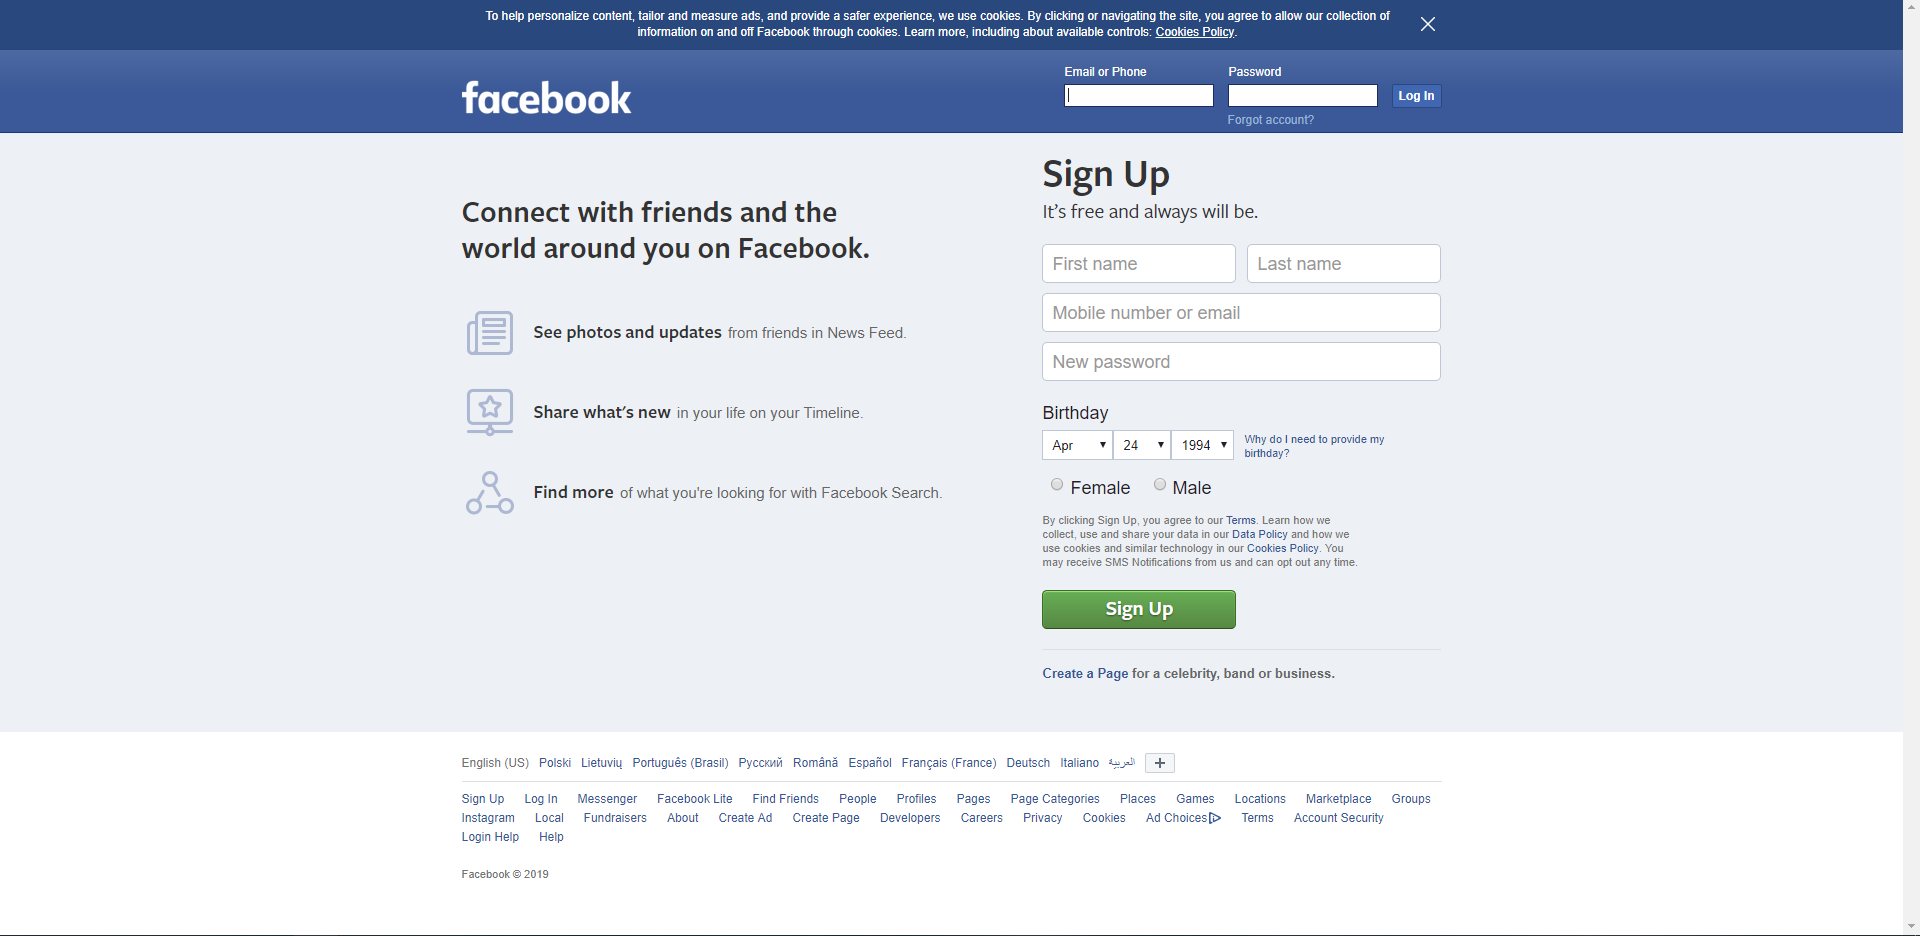
\includegraphics[width=.9\linewidth]{img/facebookCSS.PNG}
      \captionof{figure}{CSS Facebook}
      \label{fig:aboutPC}
    \end{minipage}%
    \begin{minipage}{.50\textwidth}
      \centering
      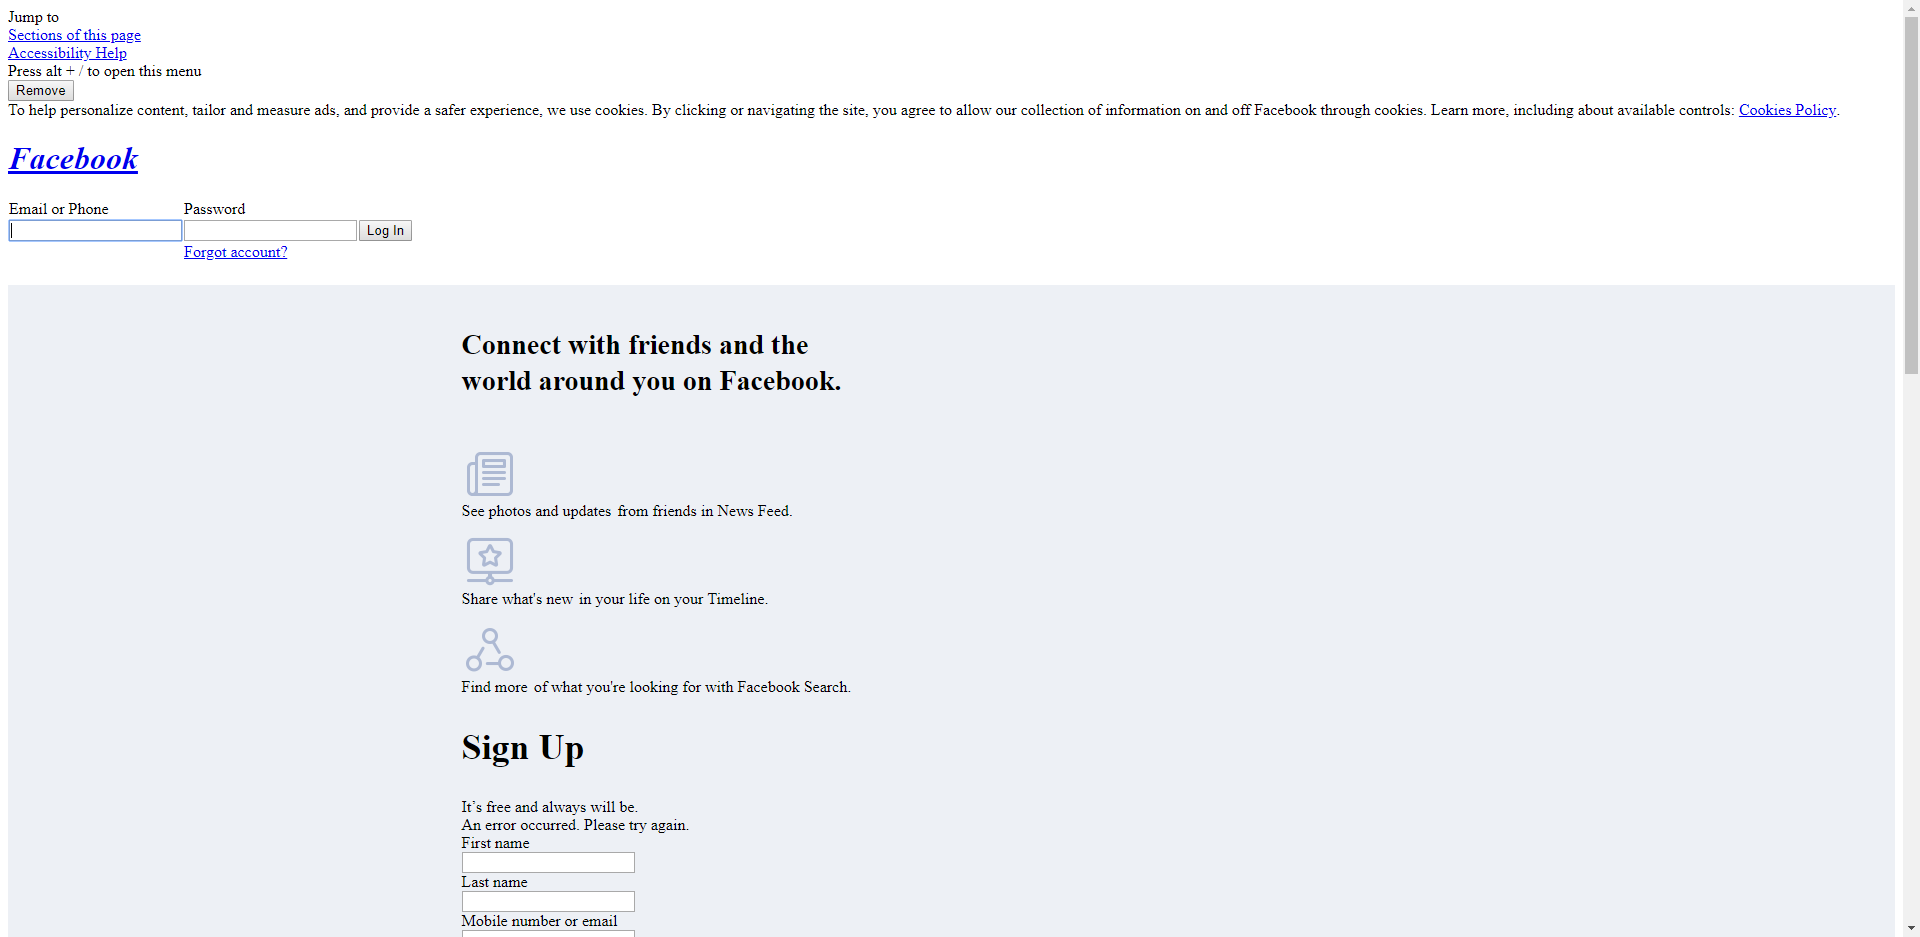
\includegraphics[width=.9\linewidth]{img/facebookNoCSS.PNG}
      \captionof{figure}{No CSS Facebook}
      \label{fig:aboutMobile}
    \end{minipage}
\end{figure}

As we can see above is an example of what the web would look like without CSS. Facebook would go from a modern looking website to a very basic text website with a few images spread around.

CSS is an extremely easy tool to grasp, but takes time to master, especially with the different screen sizes, aspect ratios and resolutions.

\subsection{Bootstrap}
Bootstrap is a pre-written library of CSS files that enables developers to rapidly develop the UI for their website. Bootstrap also allows developers to make their own CSS files and build on top of Bootstrap to refine a website design.

Bootstrap is great for quickly developing prototypes for website as it takes a lot of the grunt work and allows the developer to concentrate on getting the functionality right. CSS offers a great way to style a website, but often it can be hard to get a certain function to work correctly. Bootstrap takes care of a lot of the functionality the developer may need such as a sticky navigation-bar. Instead of the developer making a their own sticky navigation-bar using CSS and JavaScript, they can off-load that work to Bootstrap which will do all that using the specified Bootstrap class.

\subsection{Angular Material}
Angular Material is developed bu Google and was developed to meet the demand of their new design spec 'Google Now'. Google Now laid out a grid-based website with animations and responsive cards, which was used used until the serviced was discontinued.

\begin{displayquote}
"Unlike real paper, our digital material can expand and reform intelligently. Material has physical surfaces and edges. Seams and shadows provide meaning about what you can touch" - Matias Duarte, VP of Design at Google
\end{displayquote}

Angular Material was birthed from the now defunct service. Angular Material was made to create a Bootstrap like alternative. Although Angular Material is an alternative to Bootstrap to develop front-end user interfaces, Bootstrap is often used in conjunction with Angular Material.

% ========================== Other Technology's  ========================== 
\section{Other Technologies/Development environment}
In this section we will go over the technologies we used to develop and test the web application.

\subsection{Visual Studio Code}
\begin{figure}[H]
  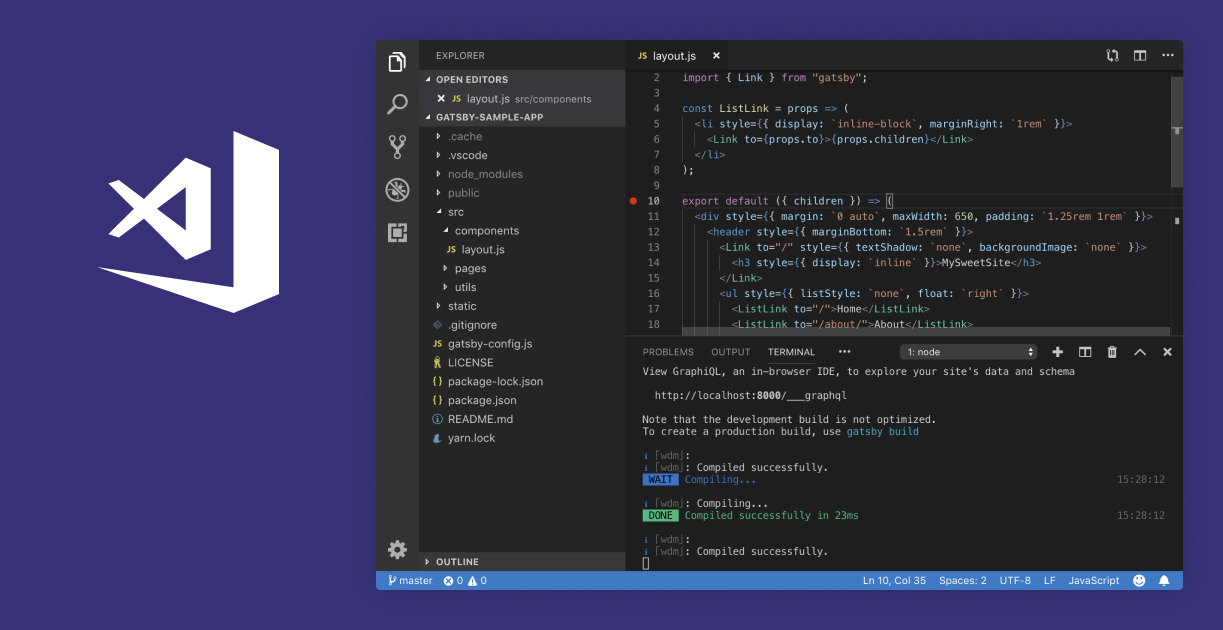
\includegraphics[width=\linewidth]{img/opengraph-home.png}
  \caption{Visual Studio Code View}
  \label{fig:VSC}
\end{figure}

Use used Microsoft's Visual Studio Code as an integrated development environment as it was perfect for what we needed. We needed an integrated development environment that didn't just support one language. We needed one that supported, JavaScript, TypeScript, HTML, CSS and LaTeX. Visual Studio Code offers a specialized extensions that make developing with these technologies more initiative.

\subsubsection{Extensions}
Extensions for Visual Studio Code are add-ons developed by others to make the development environment in Visual Studio Code better for a specific task.

\paragraph{HTML CSS Support}
HTML CSS Support extension is just what it sounds like, it adds better support for HTML and CSS in Visual Studio Code. Although you can easily write code in Visual Studio Code for HTML and CSS this extension adds features that make the development of HTML and CSS like developing Java using Eclipse would.

\begin{itemize}
    \item Class attribute completion
    \item Id attribute completion.
    \item Supports Zen Coding completion for class and id attributes.
    \item Scans workspace folder for CSS and SCSS files.
    \item Supports remote CSS files.
\end{itemize}

It's small features like these that make developing HTML and CSS a little easier, especially when developing a full stack website. HTML CSS Support extension made developing with HTML and CSS feel more natural in Visual Studio Code.

\paragraph{JavaScript (ES6) Code Snippets}
JavaScript (ES6) Code Snippets is an extension which adds shortcuts for common JavaScript and Typescript functionality such as for loop, console log and class constructors.

Supports:
\begin{itemize}
    \item JavaScript (.js)
    \item TypeScript (.ts)
    \item JavaScript React (.jsx)
    \item TypeScript React (.tsx)
    \item Html (.html)
    \item Vue (.vue)
\end{itemize}

The extension supporting both JavaScript and TypeScript was what sold us on the extension as those two languages made up the majority of our code-base. 

Using the extension is very easy once you know a few of the shortcuts and how to use them. An example of use would be typing 'clg' and pressing TAB which would convert 'clg' to 'console.log();'. The extension made getting something setup easy such as 'fof' and pressing TAB becoming 'for(const item of object) {}'. Although very basic, it made writing small code snippets easier and more in line with IDEs such as Eclipse with 'sysout' and then pressing CTRL-SPACE which produced 'System.out.println'.

\paragraph{LaTeX Workshop}
LaTeX Workshop was used early on in development. The extension provided live PDF view to see how changes looked and has came with quality of life features such as shortcuts.

LaTeX Workshop made developing LaTeX in Visual Studio Code easier with the features it provided.

\subsection{Browsers}
We used two primary and popular browsers during development. We didn't want to just use one as a feature might work for one but not the other. This wasn't a big problem as Angular handled much of the primary features with each browser, the bigger problem with trying to get cross browser support was CSS settings and how each browser would interpret them. We used chrome, Internet Explorer/Edge and Firefox as they had the largest market-share.